\documentclass[12pt]{article}
\usepackage[spanish,activeacute]{babel}
\usepackage{graphicx}
\usepackage{wrapfig}
\usepackage[utf8]{inputenc}
\usepackage[margin=3cm]{geometry}
\usepackage{hyperref} 

\begin{document}


\begin{picture}(18,4)
\put(50,-220){
\includegraphics[width=10cm,height=5cm]{fiec}}
\end{picture}

\begin{center}


\textbf{{\Huge Escuela Superior Politécnica del Litoral}\\[7cm]
{\LARGE Lenguajes de Programación}}\\[3.5cm]

{\LARGE \textbf{Manual de Usuario}}\\[1.5cm]
{\large Gabriel Aumala \\Wilson Enríquez\\ Kevin Zambrano}\\[2cm]
Ingeniería en Ciencias Computacionales\\[1cm]
Guayaquil - \today
\end{center}



\title{\bfseries\Huge Buscaminas  - Android\\ Manual de usuario}

\date{}



\begin{minipage}{0.55\textwidth}
\begingroup
\let\center\flushleft
\let\endcenter\endflushleft
\maketitle

\endgroup
\end{minipage}
\begin{minipage}{0.1\textwidth}
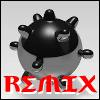
\includegraphics[height=6cm,width=6cm]{minas} 


\end{minipage}





\section{Introducción}

El proyecto consiste en elaborar una versión del juego “Buscaminas” que sea compatible con dispositivos Android. El juego debe incluir diferentes niveles de dificultad y un ranking para los jugadores basado en el tiempo que les toma ganar la partida.




\section{Alcance}

	La versión actual del proyecto es totalmente funcional, incluye 3 tableros para dificultades fácil, media y difícil. La aplicación también tiene un modo “Remix” con reglas modificadas para obtener una experiencia más ágil e intuitiva de juego. 

	

\section{Problemas Resueltos}
	Entre las dificultades que encontramos al programar para Android, una de ellas fue la implementación de la función para abrir celdas adyacentes al hacer click en un espacio que no tenga minas a su alrededor. Para crear esta función utilizamos recursividad y verificamos varias condiciones para determinar los espacios adyacentes, la dificultad principal estaba en que trabajamos con un arreglo de una sola dimensión para los botones. 
\\Se solucionó ciertos problemas de compatibilidad con modelos de tablets de pocos recursos y tablets de última generación. Para esto, tuvimos que modificar los assets acorde a las distintas resoluciones que poseen los dispositivos.
\\Otro de los problemas que encontramos fue alcanzar un balance para el modo “Remix” del juego. Tuvimos que diseñar las mecánicas de manera que hicieran el juego más divertido, que sean lo suficientemente relevantes a la acción y que no se perdiera la esencia que hace  al juego lo que es. 

	
\section{Experiencias trabajando con Android}
Trabajar con Android ha sido una experiencia valiosa, ya que es uno de los mercados más concurridos en la actual y tener nociones de programación para este sistema operativo nos ayudará en nuestra vida profesional. Una de las ventajas de trabajar con Android es la cantidad de información disponible para los usuarios. \\Gracias a la cantidad de tutoriales e información relacionada a Android, se nos facilitó bastante el desarrollo del proyecto, aunque esta fue una de las primeras ocasiones en que trabajamos para esta plataforma.
\\Entre los problemas que encontramos, fue que había que modificar las imágenes para varias resoluciones, ya que si no se crean problemas de compatibilidad con la diversa cantidad de equipos que utilizan esta plataforma.
\\Otro problema que encontramos fue que a medida que avanzan las versiones de Android, se han agregado funciones que no estaban disponibles en versiones anteriores. Debido a esto no implementamos las banderas con el método “Drag and Drop”, ya que no está nos daba problemas en la versión 2.3 de Android, que fue la que principalmente usamos para programar.

\section{Conclusiones}
Este proyecto resultó ser más laborioso de lo esperado, a pesar de que diseñar la lógica del juego y programarla fue sencillo. Tomo tiempo adaptarnos a Android y en varias ocasiones surgieron problemas, pero gracias a la gran cantidad de información disponible, encontramos soluciones a la mayoría de estos problemas. 
\\A pesar de las dificultades encontradas durante la realización del proyecto, completar el mismo no fue lo más difícil. Lo que ha dado más trabajo ha sido realizar mejoras al proyecto, sea en la interfaz gráfica, añadiéndole sonidos, o simplemente corrigiendo partes del código. Al ser una aplicación dirigida a Android, se espera que tenga una interfaz amena para los consumidores, esto nos impulsa a realizar constantemente mejoras al proyecto. 
\\Todo esto fue una gran experiencia que contribuirá mucho a nuestras carreras profesionales, ya que el mercado de Android sigue en auge y el familiarizarnos con este entorno será muy útil. 

\section{Screenshots}

\subsection{Fácil}

\begin{minipage}{0.1\textwidth}
\includegraphics[height=6cm,width=12cm]{facil} 
\end{minipage}

\begin{minipage}{0.1\textwidth}
\includegraphics[height=6cm,width=12cm]{facil2} 
\end{minipage}

\begin{minipage}{0.1\textwidth}
\includegraphics[height=6cm,width=12cm]{facil3} 
\end{minipage}

\subsection{Difícil}

\begin{minipage}{0.1\textwidth}
\includegraphics[height=6cm,width=12cm]{dificil} 
\end{minipage}

\subsection{Remix}

\begin{minipage}{0.1\textwidth}
\includegraphics[height=6cm,width=12cm]{remix} 
\end{minipage}

\begin{minipage}{0.1\textwidth}
\includegraphics[height=6cm,width=12cm]{remix2} 
\end{minipage}

\begin{minipage}{0.1\textwidth}
\includegraphics[height=6cm,width=12cm]{remix3} 
\end{minipage}

\begin{minipage}{0.1\textwidth}
\includegraphics[height=6cm,width=12cm]{remix4} 
\end{minipage}


		
		



		


\end{document}